% Figure 1 of GL(K)_attention_v2.tex (fig:link_construction): statistical sections, frames, and a group link.
% Extracted verbatim from the manuscript's tikzpicture. Build (TeX Live 2025, from this directory):
%   pdflatex -interaction=nonstopmode bundle_geometry.tex
%   pdftoppm -r 330 -png -singlefile bundle_geometry.pdf bundle_geometry
\documentclass[border=8pt]{standalone}
\usepackage[T1]{fontenc}
\usepackage{lmodern}
\usepackage{amsmath,amssymb}
\usepackage{xcolor}
\usepackage{tikz}
\usetikzlibrary{calc, arrows.meta, positioning}
\newcommand{\softmax}{\mathrm{softmax}}
\newcommand{\KL}{\mathrm{KL}}
\newcommand{\Tr}{\mathrm{Tr}}
\begin{document}
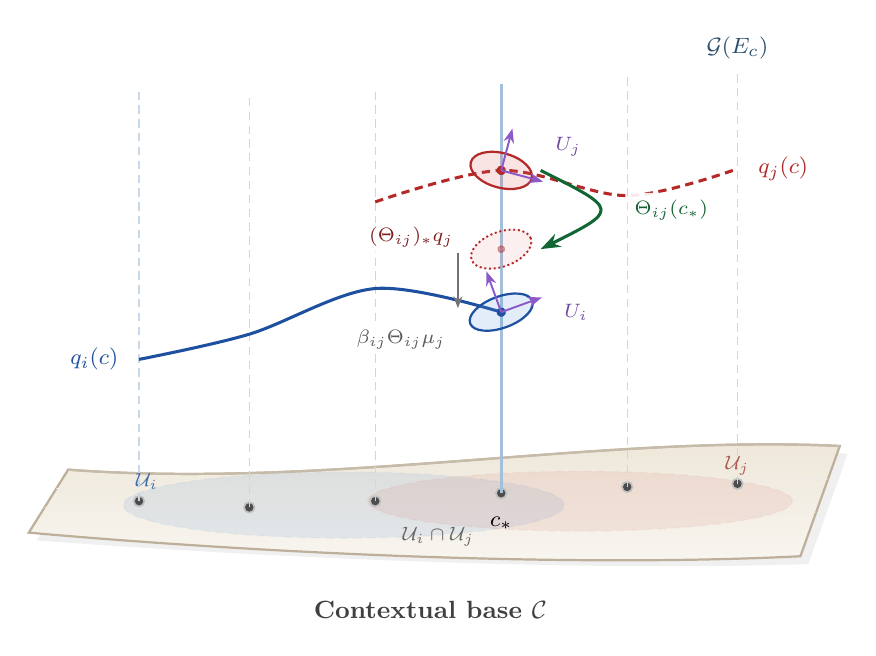
\begin{tikzpicture}[ every node/.style={font=\small}]

\definecolor{fiberblue}{RGB}{70,130,180}
\definecolor{sectionblue}{RGB}{30,80,160}
\definecolor{sectionred}{RGB}{180,40,40}
\definecolor{transportgreen}{RGB}{20,120,60}
\definecolor{gaussblue}{RGB}{100,150,220}
\definecolor{gaussred}{RGB}{220,100,100}
\definecolor{framecol}{RGB}{140,90,200}
\definecolor{basetan}{RGB}{230,220,200}
\definecolor{baseedge}{RGB}{160,140,110}
\definecolor{neighborblue}{RGB}{80,140,210}
\definecolor{neighborred}{RGB}{210,110,100}

\path
  (-0.3,0.1) coordinate (M1)
  (9.5,0.4) coordinate (M2)
  (9.0,-1.0) coordinate (M3)
  (-0.8,-0.7) coordinate (M4);

\filldraw[fill=black!6, draw=none]
  ($(M1)+(0.1,-0.1)$)
  .. controls (3.0,-0.2) and (6.5,0.6) .. ($(M2)+(0.1,-0.1)$)
  -- ($(M3)+(0.1,-0.1)$)
  .. controls (6.0,-1.2) and (2.0,-1.0) .. ($(M4)+(0.1,-0.1)$)
  -- cycle;

\shade[top color=basetan!70, bottom color=basetan!25, draw=baseedge!70, thick]
  (M1)
  .. controls (3.0,-0.15) and (6.5,0.55) .. (M2)
  -- (M3)
  .. controls (6.0,-1.15) and (2.0,-0.95) .. (M4)
  -- cycle;

\draw[baseedge!60, thick]
  (M1) .. controls (3.0,-0.15) and (6.5,0.55) .. (M2);

\foreach \t in {0.3, 0.6} {
  \draw[baseedge!15, very thin]
  ($(M1)!\t!(M4)$) .. controls
  ($($(M1)!\t!(M4)$)!0.4!($(M2)!\t!(M3)$)+(0,0.04)$) and
  ($($(M1)!\t!(M4)$)!0.6!($(M2)!\t!(M3)$)+(-0.02,-0.04)$)
  .. ($(M2)!\t!(M3)$);
}

\node[below, black!75, font=\small\bfseries] at (4.3,-1.45) {Contextual base $\mathcal{C}$};

\coordinate (C1) at (0.6,-0.30);
\coordinate (C2) at (2.0,-0.38);
\coordinate (C3) at (3.6,-0.30);
\coordinate (C4) at (5.2,-0.20);
\coordinate (C5) at (6.8,-0.12);
\coordinate (C6) at (8.2,-0.08);


\filldraw[neighborblue, opacity=0.12, draw=neighborblue!60,
  line width=0.5pt, densely dashed]
  (3.2,-0.35) ellipse (2.8 and 0.42);
\node[neighborblue!80!black, font=\scriptsize] at (0.7,-0.05) {$\mathcal{U}_i$};

\filldraw[neighborred, opacity=0.12, draw=neighborred!60,
  line width=0.5pt, densely dashed]
  (6.2,-0.30) ellipse (2.7 and 0.38);
\node[neighborred!80!black, font=\scriptsize] at (8.2,0.15) {$\mathcal{U}_j$};

\node[black!60, font=\scriptsize] at (4.4,-0.75) {$\mathcal{U}_i \cap \mathcal{U}_j$};

\foreach \c in {C1,C2,C3,C4,C5,C6} {
  \filldraw[black!25] (\c) circle (2pt);
  \filldraw[black!70] (\c) circle (1.3pt);
}

\pgfmathsetmacro{\fh}{5.2}

\foreach \c in {C1,C2,C3,C4,C5,C6} {
  \draw[fiberblue!30, densely dashed, line width=0.4pt]
  (\c) -- ++(0,\fh);
}

\node[above=2pt, fiberblue!60!black, font=\footnotesize]
  at ($(C6)+(0,\fh)$) {$\mathcal{G}(E_c)$};


\coordinate (Si1) at ($(C1)+(0,1.8)$);
\coordinate (Si2) at ($(C2)+(0,2.2)$);
\coordinate (Si3) at ($(C3)+(0,2.7)$);
\coordinate (Si4) at ($(C4)+(0,2.3)$);

\draw[sectionblue, line width=1.1pt]
  plot[smooth, tension=0.55] coordinates {
  (Si1) (Si2) (Si3) (Si4)
  };

\coordinate (Sj3) at ($(C3)+(0,3.8)$);
\coordinate (Sj4) at ($(C4)+(0,4.1)$);
\coordinate (Sj5) at ($(C5)+(0,3.7)$);
\coordinate (Sj6) at ($(C6)+(0,4.0)$);

\draw[sectionred, densely dashed, line width=1.1pt]
  plot[smooth, tension=0.55] coordinates {
  (Sj3) (Sj4) (Sj5) (Sj6)
  };

\node[sectionblue, font=\footnotesize, left=4pt] at (Si1) {$q_i(c)$};
\node[sectionred, font=\footnotesize, right=4pt] at (Sj6) {$q_j(c)$};


\draw[fiberblue!50, line width=1.0pt] (C4) -- ++(0,\fh);

\node[below=5pt, black, font=\footnotesize\itshape] at (C4) {$c_*$};


\begin{scope}[shift={(Si4)}, rotate=20]
  \filldraw[gaussblue, opacity=0.18] (0,0) ellipse (0.42 and 0.20);
  \draw[sectionblue, line width=0.8pt] (0,0) ellipse (0.42 and 0.20);
  \filldraw[sectionblue] (0,0) circle (1.5pt);
\end{scope}

\begin{scope}[shift={(Sj4)}, rotate=-15]
  \filldraw[gaussred, opacity=0.18] (0,0) ellipse (0.40 and 0.22);
  \draw[sectionred, line width=0.8pt] (0,0) ellipse (0.40 and 0.22);
  \filldraw[sectionred] (0,0) circle (1.5pt);
\end{scope}


\begin{scope}[shift={(Si4)}, rotate=20]
  \draw[-{Stealth[length=1.8mm]}, framecol, line width=0.7pt]
  (0,0) -- (0.55,0);
  \draw[-{Stealth[length=1.8mm]}, framecol, line width=0.7pt]
  (0,0) -- (0,0.55);
\end{scope}
\node[framecol!80!black, font=\scriptsize] at ($(Si4)+(0.95,0.0)$) {$U_i$};

\begin{scope}[shift={(Sj4)}, rotate=-15]
  \draw[-{Stealth[length=1.8mm]}, framecol, line width=0.7pt]
  (0,0) -- (0.55,0);
  \draw[-{Stealth[length=1.8mm]}, framecol, line width=0.7pt]
  (0,0) -- (0,0.55);
\end{scope}
\node[framecol!80!black, font=\scriptsize] at ($(Sj4)+(0.85,0.30)$) {$U_j$};


\coordinate (Ghost) at ($(Si4)+(0,0.8)$);
\begin{scope}[shift={(Ghost)}, rotate=20]
  \filldraw[gaussred, opacity=0.10] (0,0) ellipse (0.40 and 0.22);
  \draw[sectionred, densely dotted, line width=0.7pt] (0,0) ellipse (0.40 and 0.22);
  \filldraw[sectionred, opacity=0.4] (0,0) circle (1.2pt);
\end{scope}

\node[sectionred!70!black, font=\scriptsize,
  fill=white, fill opacity=0.9, text opacity=1,
  inner sep=1.5pt, rounded corners=1pt, anchor=east]
  (pushforwardlabel) at ($(Ghost)+(-0.55,0.15)$) {$(\Theta_{ij})_*q_j$};

\draw[-{Stealth[length=2.5mm, width=1.8mm]},
  transportgreen!85!black, line width=1.1pt]
  ($(Sj4)+(0.5,0)$)
  .. controls ($(Sj4)+(1.5,-0.5)$) and ($(Ghost)+(1.5,0.5)$)
  .. ($(Ghost)+(0.5,0)$);

\node[transportgreen!80!black, font=\scriptsize\bfseries,
  fill=white, fill opacity=0.9, text opacity=1,
  inner sep=2.5pt, rounded corners=2pt, anchor=west]
  at ($(Sj4)!0.5!(Ghost)+(1.6,0)$) {$\Theta_{ij}(c_*)$};


\draw[-{Stealth[length=1.5mm]},
  black!55, line width=0.6pt]
  ($(Ghost)+(-0.55,-0.05)$) -- ($(Si4)+(-0.55,0.05)$);

\node[black!65, font=\scriptsize,
  fill=white, fill opacity=0.9, text opacity=1,
  inner sep=1.5pt, rounded corners=1pt, anchor=east]
  (messagelabel) at ($(Si4)+(-0.65,-0.35)$) {$\beta_{ij}\Theta_{ij}\mu_j$};

\end{tikzpicture}
\end{document}
